\section{Prompt Template Engineering}
\label{sec:template}

Prompt template engineering involves creating templates to provide input, or ``prompts,'' to a language model to guide its output generation. In this section, we discuss prompt template engineering methods for basic building blocks, and then integrate the methods of definition, elenchus, dialectic, maieutics, and counterfactual reasoning to compose more complex templates. We present experimental results using different types of documents to demonstrate how the Socratic method can improve the accuracy and conciseness of the output through arguments and verification, as well as facilitate guided generalization and creativity.

\subsection{Basic, One Shot Template}

Let's begin by discussing a simple one-shot prompt template. In the work of \cite{SocraticModels-Google2022}, a simple formulation function is used to generate the prompt $x'$, which is obtained by applying the function $f_{prompt}(x)$ to the input $x$.

For machine translation, the prompt template can take the form of ``Translate from [Lan$_{from}$]: [X] to [Lan$_{to}$]: [Y],'' where Lan$_{from}$ can be either detected by the prompt template or identified by the LLM. The input $x$ provides the information to fill in the slots [X] and [Lan$_{to}$]. For example, if the input is ``translate good morning to French,'' the prompt template $x'$ would be ``Translate from English: 'good morning' to French: [Y].'' The empty slot [Y] is then filled with the LLM's output, such as ``bonjour.'' In cases where the LLM produces multiple responses, it can also provide a score for each, which the prompt template can use to select the highest-scoring response or to request a summary from the LLM.


There are three main design considerations when engineering a basic prompt. 
\begin{noindenumerate}
\item {Input style}. It is important to consider how to phrase the template so that it can handle different styles of user input for the same task. For example, a user may ask for a translation task to be performed by saying ``Translate $x$ to French,'' or ``What is the French translation of $x$?''
\item {LLM capability}. As discussed in \cite{PromptSurvey2023}, it is important to take into account the patterns and capabilities of the partner language model (LLM) when designing the template, such as whether the LLM is left-to-right \cite{OpenAI-GPT3-2020} or masked \cite{Devlin2019BERTPO}.
\item {Cost}. Certain tasks, such as language detection and summarization, can be performed by the template itself or by the LLM. The decision of whether to perform a task within the prompt template or to use the LLM should be based on factors such as cost.
\end{noindenumerate}

To address the first two technical challenges, one can start by hand-engineering a few seed templates and then paraphrasing them into an ensemble \cite{Haviv2021BERTeseLT}. We believe that the basic, one-shot formulation can always be replaced by an ensemble formulation \cite{Peng2022ModelEI, Schick2020ExploitingCF} and then learn the weights of its members for each query instance to produce the final output. Additionally, by examining which basic prompts have high weights, an ensemble with various paraphrased prompts can identify what an LLM knows, which can help infer its strengths without having to conduct capability
mining on the LLMs.

%\noindent
%{\color{blue} Note} Experiment idea: evaluate LLMs using ensembles.

\subsection{Prompt Clarification with Method Definition}
\label{sec:template-definition}

There are computer algorithms that can already be used to recursively clarify a question, its definitions, and sub-terms' definitions. In fact, the natural language processing (NLP) community has developed a large 
number of useful methods and algorithms over the years \cite{NLP-Text-JM3}. 
One can use NLP techniques, such as dependency parsing and named-entity recognition (NER) \cite{NLPScratch2011}, to analyze the structure and meaning of a question and identify key terms and concepts. For example, 
NER can be used to extract entities in user input, such as names, locations, and organizations, and co-reference resolution can be used to understand the referred entity of a pronoun. 
Before submitting a template to an LLM, the application (e.g., a chatbot) 
that uses the template should check if all input slots are filled, 
and perform a sanity check. In the translation example, if the [Lan$_{to}$] was not provided or the specified language is not supported by the LLM, then the application should inquire the user for clarification.

Regarding mapping a natural language input to a prompt template, existing techniques of knowledge representation and reasoning can be very helpful. More specifically, ontology alignment and semantic parsing \cite{Campagna2020AFS,zhou-etal-2021-structure} can help map an NL input to a structured representation of knowledge and infer implicit concepts and relationships. These algorithms can be used to generate more precise and accurate prompts for LLMs, and to improve the effectiveness of the Socratic method in dialogue formulation \cite{DialoguewithAttention2023}. Some available tools include NLTK (Natural Language Toolkit) and spaCy for NLP\footnote{spaCy (https://spacy.io/)}, and TensorFlow for ML\footnote{TensorFlow (https://www.tensorflow.org/)}.

%\noindent
%{\color{blue} Note} Experiment idea: compare w/ and w/o.

\subsection{Prompt Verification with Method Elenchus}

The main purposes of conducting cross examination in a template are to validate the credibility of the information sources and to identify inconsistencies in the process. Cross examination is typically conducted through a multi-turn dialogue \cite{DialoguewithAttention2023}. In the context of template engineering, the goal is to formulate a productive dialogue that can be used to assess the reliability of an LLM's output.  

There are several methods that can be used to assess and strengthen the reliability of an LLM's output. 1) The first approach is to paraphrase a question in order to obtain different answers and identify inconsistencies, if they exist, in multiple answers. 2) The second method is to ask for further evidence, such as querying top-k sources of information and asking the LLM to rate the credibility of each source. This can be used to compute the reliability of the output. 3) Additionally, template engineering can be used to query an LLM for opposing views of its output, including sources and credibility, and then evaluate if a different perspective is strong.

The implementation of the first two methods for cross examination, paraphrasing a question and asking for further evidence, is readily covered by the techniques enumerated in Section~\ref{sec:template-definition}. To implement the third method of asking for different perspectives, a simple approach is to find the sentiment of the original question and then rewrite the question with an opposite sentiment. For example, if the original question is phrased in a positive tone, the prompt template can reformulate the question with a negative tone to elicit a contrasting viewpoint.
A more elaborate method is to identify the people and sources in the LLM-generated responses and then re-post the questions to those who have a reputation for having different views. For example, if the original answer came from a democratic right-leaning source, the prompt template may post the same question to a source of a republican-left persuasion, and vice versa. This approach allows for a more comprehensive examination of the topic by considering multiple perspectives.

The template to examine the semantic relation between two sentences $S_1$ and $S_2$ can be 
written as ``<$S_1$>, [R], [$S_2$],'' where R
is one of the three most important 
types of semantic relations: paraphrase, entailment, and contradiction \cite{PTRSUN2021}. Two sentences that have the same meaning are called paraphrases of each other. Two sentences that
have different meanings can be called 
disagreement or contradiction. The template 
can be trained to identify the degree
of agreement (or disagreement) between two
sentences.  


Table \ref{tab:Elenchus} shows two examples of this. In the first example (shown on the top portion of the table), the prompter asks GPT-3 to confirm if James Watson and Francis Crick are the only contributors to the discovery of the DNA double helix structure. GPT-3 replies by mentioning two other contributors. The second example in the table asks GPT-3 to provide not only the answer to a question but also its information sources and rate the credibility of each source according to the prompter's specification. Although the reliability of GPT-3's ratings remains to be validated, this rating mechanism can serve as an alert when some sources are found to be unreliable.


\begin{table}[htbp!]
%\vspace{-.12in}
%\resizebox{\textwidth}{!}
\begin{tikzpicture}
\begin{small}
\node (table) [inner sep=0.1pt] {
\begin{tabular}{p{1.0cm}|p{6.6cm}}
\toprule
Role & Dialogue \\
\midrule
Prompt & {The discovery of the double helix structure of DNA was credited to James Watson and Francis Crick. However, are there opposing opinions to the list of contributors regarding this discovery?}\\

GPT3 & {There are some historical debates on the contributions of other scientists who also worked on the structure of DNA such as Maurice Wilkins and Rosalind Franklin.} \\ 
\midrule 

Prompt & 
{What is the tallest building in the world.  Please provide three references and rate their credibility as high, medium, or low.} \\

GPT3 & {As of 2021, the tallest building in the world is the Burj Khalifa located in Dubai, United Arab Emirates. It stands at 828 meters (2,722 feet) tall.

References:
\begin{noindenumerate}
\item Credibility {\color{red}High}: ``Burj Khalifa.''... 
 this is the official website of the building, providing accurate information.
\item Credibility {\color{red}High}: ``The Tallest Buildings in the World.'' Council on Tall Buildings and Urban Habitat... this is a well-respected organization in the field of tall building and urban habitat research.
\item Credibility {\color{red}Medium}: ``The Tallest Buildings in the World.'' World Atlas..., 
this is a well-known website providing accurate information on different topics, but it's always good to cross-reference with other sources.
\end{noindenumerate}
} \\
\bottomrule
\end{tabular}
};
\draw [rounded corners=.5em] (table.north west) rectangle (table.south east);
\end{small}
\end{tikzpicture}
\caption{Examples of Method Elenchus.}
\label{tab:Elenchus}
\vspace{-.1in}
\end{table}


\subsection{Prompt Generalization with Method Maieutics}


\begin{table}[htbp]
%\resizebox{\textwidth}{!}
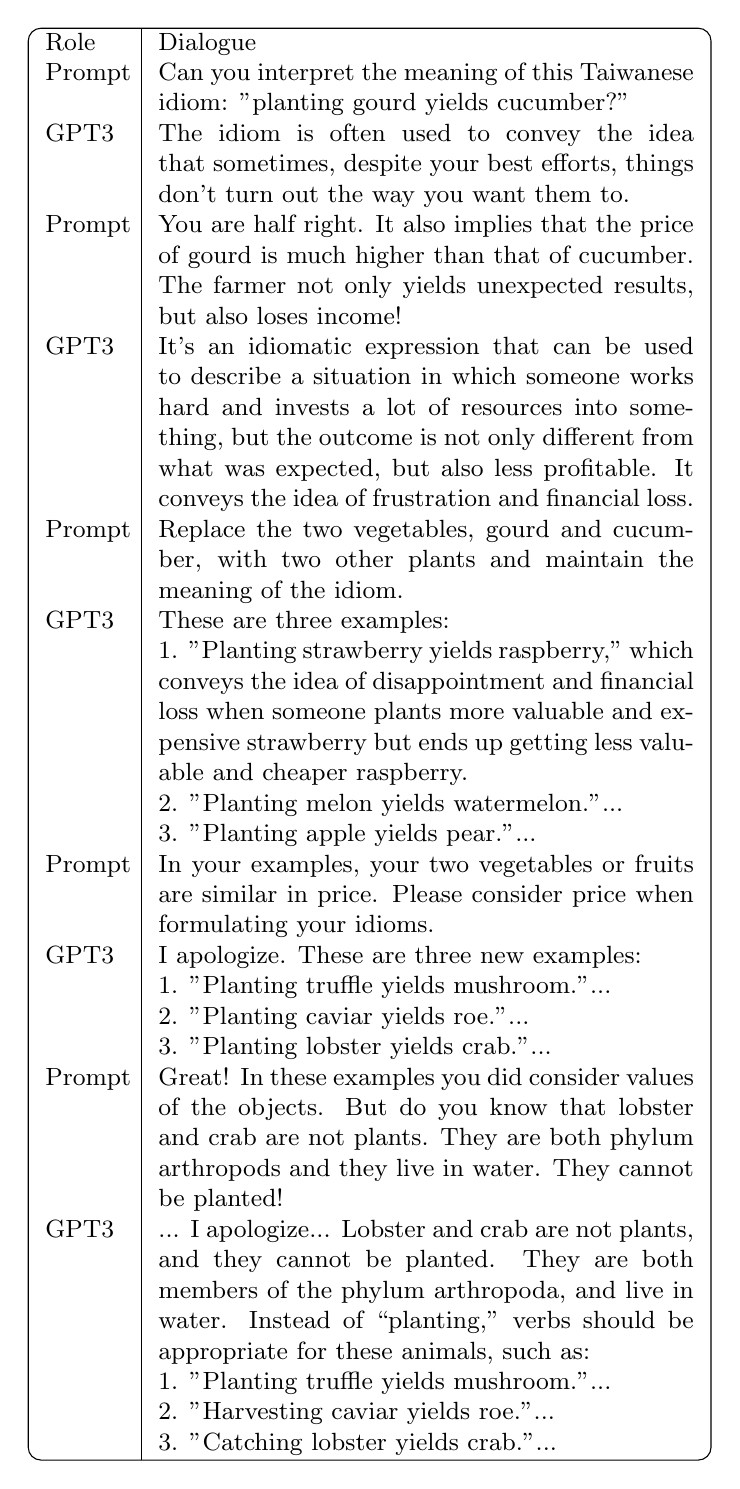
\begin{tikzpicture}
\begin{small}
\node (table) [inner sep=0pt] {
%\setlength\tabrowsep{1.5pt}
\begin{tabular}{p{1.0cm}|p{6.8cm}}
\toprule
Role & Dialogue \\
\midrule
Prompt & {Can you interpret the meaning of this Taiwanese idiom: "planting gourd yields cucumber?"}\\
GPT3 & {The idiom is often used to convey the idea that sometimes, despite your best efforts, things don't turn out the way you want them to.} \\
Prompt & {You are half right. It also implies that the price of gourd is much higher than that of cucumber. The farmer not only yields unexpected results, but also loses income! } \\

GPT3 & {It's an idiomatic expression that can be used to describe a situation in which someone works hard and invests a lot of resources into something, but the outcome is not only different from what was expected, but also less profitable. It conveys the idea of frustration and financial loss.} \\

Prompt & {Replace the two vegetables, gourd and cucumber, with two other plants and maintain the meaning of the idiom.} \\

GPT3 & {These are three examples:} \\
& 1. "Planting strawberry yields raspberry," which
conveys the idea of disappointment and financial loss when someone plants more valuable and expensive strawberry but ends up getting less valuable and cheaper raspberry. \\
& 2. "Planting melon yields watermelon."... \\
& 3. "Planting apple yields pear."... \\

Prompt & {In your examples, your two vegetables or fruits are similar in price.  Please consider price when
formulating your idioms.} \\

GPT3 & {I apologize. These are three new examples:} \\
& 1. "Planting truffle yields mushroom."... \\
& 2. "Planting caviar yields roe."... \\
& 3. "Planting lobster yields crab."... \\

Prompt & {Great! In these examples you did consider values of the objects. But do you know that lobster and crab are not plants. They are both phylum arthropods and they live in water. They cannot be planted! }  \\

GPT3 & {... I apologize... Lobster and crab are not plants, and they cannot be planted. They are both members of the phylum arthropoda, and live in water. Instead of ``planting,'' verbs should be appropriate for these animals, such as:} \\
& 1. "Planting truffle yields mushroom."... \\
& 2. "Harvesting caviar yields roe."... \\
& 3. "Catching lobster yields crab."... \\
\bottomrule
\end{tabular}
};
\draw [rounded corners=.5em] (table.north west) rectangle (table.south east);
\end{small}
\end{tikzpicture}
\caption{Example of Method Maieutics.}
\vspace{-.1in}
\label{tab:Maieutics}
\vspace{-.15in}
\end{table}


The example shown in Table~\ref{tab:Maieutics}, ``planting gourd yields cucumber,'' requires GPT-3 to first learn to select two produce objects, either vegetables or fruit, as input. The template is ``The farmer was so sad because he [verb] [X] but yields [Y], where price(X) >> price(Y).'' The first attempt may not strongly convey the condition price(X) >> price(Y), but with a few training iterations, GPT-3 started to ``recognize'' the price constraint and could also provide justifications when arguing for the price of tea being much higher than the price of spinach (not presented in the table).

Interestingly, after GPT-3 learned the price constraint, it started suggesting food items other than produce, such as caviar, roe, lobster, and crab. While the price constraint was observed, the verb ``plant'' is incorrect. Here, we suggest making the hard-coded verb ``plant'' an output slot: ``The farmer was so sad because he [verb] [X] but yields [Y], where price(X) >> price(Y).'' Amazingly, GPT-3 is able to fill in the slot with accurate verbs:

\begin{noindlist}
\item ``Harvesting (planting) truffle yields mushroom.''
\item ``Fishing (harvesting) for caviar yields roe.''
\item ``Trapping (catching) lobster yields crab.''
\end{noindlist}

This example demonstrates that GPT-3 can generate novel examples based on a template. When it suggests food items other than produce, it could be seen as an error as the boundary set by the verb ``plant'' is violated. However, this could also be seen as an innovative act by GPT-3, extending the constraint hinted by the verb. Impressively, the new examples still preserve the original intent of showing a producer's emotional distress.

How can this guided generalization be accurately and automatically performed to edit a template? Socrates' method of generalization starts with specific instances and then draws general statements from them. The procedure for generalization involves identifying common patterns or themes in a set of examples, and then formulating a general rule that captures these patterns. In the example presented in Table~\ref{tab:Maieutics}, we started by asking GPT-3 to meet the price(X) >> price(Y) constraint, with the condition that X and Y must both be produce grown in soil. However, upon analyzing GPT-3's outputs, we discovered that some instances of X and Y were not produce (e.g., lobster and caviar). This finding led to the realization that the hard-coded verb ``plant'' in the template was too restrictive. To address this issue, we applied generalization by allowing the [verb] slot to be open, making the template statement more general. In this case, the mistakes made by GPT-3 served as valuable training data, allowing us to generalize the original template and make the expression more vivid and dynamic.

\subsection{Prompt Exploration with Counterfactual Reasoning}

Imagination and creating novel plots are crucial for writers, as it allows for ``creative freedom'' and ``artistic license.'' Creativity is the ability to think differently and approach problems with fresh and imaginative ideas.

However, an imagination without a clear subject matter, scope, or a story line can lead to a lack of productivity. To captivate the audience, a writer must consider human experiences and emotions as constraints. Therefore, ``creative freedom'' should not be viewed as total freedom, but rather as the ability to condition future narratives in the context and to create plots that turn and twist in unexpected ways.

The technique of counterfactual \cite{Pearl2009} can be useful in guiding imagination. It involves considering alternative scenarios and outcomes. This can lead to the exploration of different possibilities and the generation of new and unique plot ideas. For example, a writer may ask ``what if'' questions to change the narrative of events, such as ``what if the main character had not fallen in love?'' or ``what if an accident occurred on the way to a highly-anticipated date?'' By considering these counterfactuals, a writer and an LLM can create more engaging and interesting stories. One can ask an LLM to generate several scenarios and then select the most suitable one for the writer to continue writing.

We have experimented with using the counterfactual technique to
rewrite chapters in Chinese classical novels, ``Outlaws of the Marsh'' and ``Dream of the Red Chamber.'' We have also asked GPT-3 to rewrite Genesis chapter 3 after verse six by prompting GPT-3
that: ``What if Adam and Eve refused the serpent to eat the fruit?''
The results were interesting, as GPT-3 was able to generate unique and interesting scenarios that deviated from the original story while still maintaining the core themes and concepts. 
This technique can be used in a wide range of writing and storytelling, from fiction to non-fiction, to generate new and compelling ideas. 
The revised Genesis 3:6 is presented in the Appendix.

\section{Pilot Study}
\label{sec:pilot}

Our pilot study uses CRIT, and it aims to answer two questions:
Should all prompts be issued to GPT-3 sequentially or they
can be issued all together?  
What limitations can be identified for improvement?
The study utilizes exercises with established answers from the $8^{th}$ edition of the textbook ``Ask the Right Questions'' by the authors of \cite{AskRightQ2001}. It is important to note that the study evaluates the effectiveness of CRIT's prompt template, rather than the language models to which CRIT can issue prompts.

\begin{comment}
Table~\ref{tab:pilot1} presents two examples from \cite{AskRightQ2001}. The results of the CRIT analysis, which include conclusion extraction and reason identification, match or exceed the evaluations made by the authors. In the first example, the authors consider the document to be somewhat ambiguous with two potential conclusions. CRIT finds the document to be poorly written without a clear conclusion and gives it a low validity score of $60\%$. This low credibility score is attributed to the absence of sufficient evidence in the argument to justify two possible claims. 
In the second example, CRIT accurately extracts the claim and arguments and recognizes that the argument's validity is subjective and dependent on context such as religious beliefs and cultural perspectives. 
\end{comment}

On short documents, the results are similar in quality when CRIT is used to issue prompts either sequentially or all together as one prompt, as long as the instructions are consistent. However, when evaluating long articles in \cite{501Q2004}, CRIT issuing prompts one after another yields much higher presentation quality in both organization and clarity. 
(Due to the space limit, we document examples in a supplement document \cite{CRITExtended2023}.) In the teaching mode, the sequential option is thus much preferred. Furthermore,
When a reason is itself a claim and requires CRIT to validate its supporting references, using a sequential approach is more flexible and enables CRIT to query for references and then execute the process recursively.

\begin{table}[hbt!]
%\vspace{-.1in}
%\resizebox{\textwidth}{!}
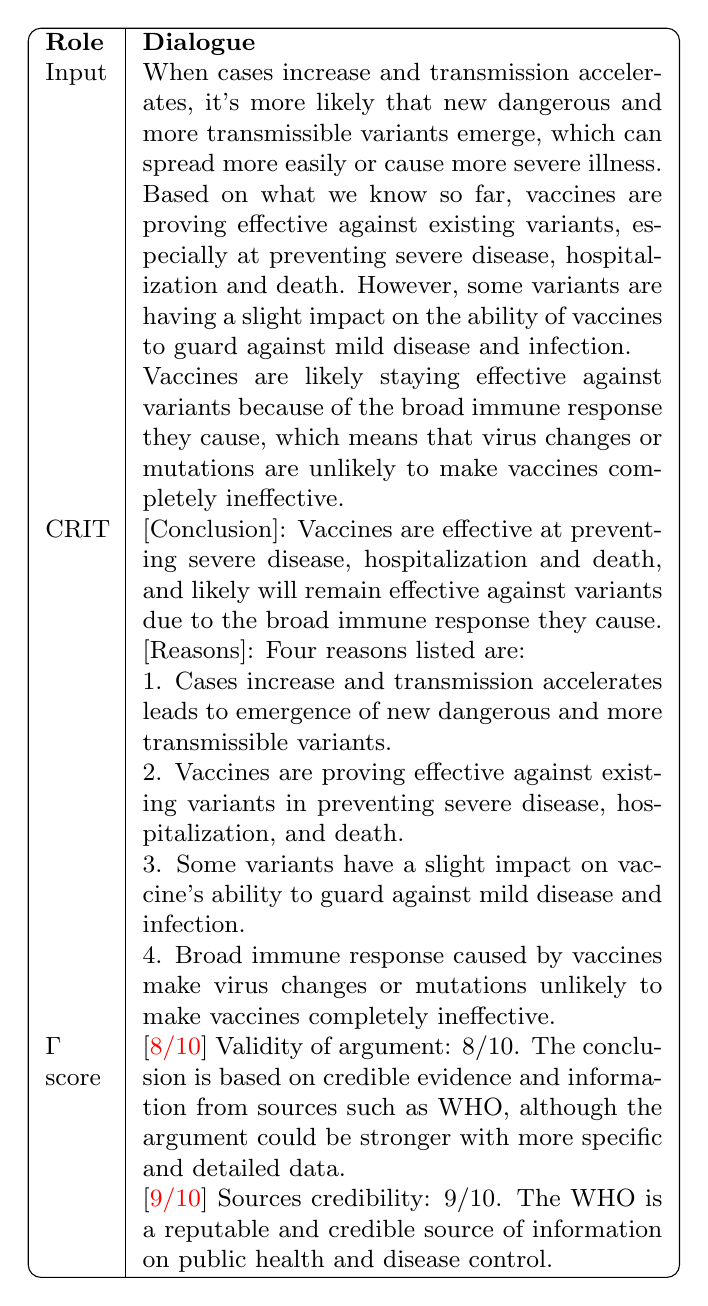
\begin{tikzpicture}
\begin{small}
\node (table) [inner sep=0pt] {
\begin{tabular}{p{0.8cm}|p{6.6cm}}
\toprule
\textbf{Role} & \textbf{Dialogue} \\
\midrule
{Input} & {When cases increase and transmission accelerates, it’s more likely that new dangerous and more transmissible variants emerge, which can spread more easily or cause more severe illness.

Based on what we know so far, vaccines are proving effective against existing variants, especially at preventing severe disease, hospitalization and death. However, some variants are having a slight impact on the ability of vaccines to guard against mild disease and infection.

Vaccines are likely staying effective against variants because of the broad immune response they cause, which means that virus changes or mutations are unlikely to make vaccines completely ineffective.} \\

{CRIT} & {[Conclusion]: Vaccines are effective at preventing severe disease, hospitalization and death, and likely will remain effective against variants due to the broad immune response they cause.} \\

& [Reasons]: Four reasons listed are: \\
& 1.  Cases increase and transmission accelerates leads to emergence of new dangerous and more transmissible variants. \\
& 2. Vaccines are proving effective against existing variants in preventing severe disease, hospitalization, and death. \\
& 3. Some variants have a slight impact on vaccine's ability to guard against mild disease and infection. \\
& 4. Broad immune response caused by vaccines make virus changes or mutations unlikely to make vaccines completely ineffective. \\
\midrule
{$\Gamma$ score} & {[{\color{red}8/10}] Validity of argument: 8/10. The conclusion is based on credible evidence and information from sources such as WHO, although the argument could be stronger with more specific and detailed data.} \\
& {[{\color{red}9/10}] Sources credibility: 9/10. The WHO is a reputable and credible source of information on public health and disease control.} \\
%\textbf{Final Score}: {\color{red}$72\%$ High} (High: above $60\%$, Low: below $25\%$)
%$} \\
\bottomrule
\end{tabular}
};
\draw [rounded corners=.5em] (table.north west) rectangle (table.south east);
\end{small}
\end{tikzpicture}
%\vspace{-.05in}
\caption{Pilot Study on CRIT. 
%WHO's post about the expected efficacy of 
%COVID vaccines on its variants.
}
\vspace{-.20in}
\label{tab:pilot2}
\end{table}

Table~\ref{tab:pilot2} presents a document about COVID-19 vaccine efficacy, published by the World Health Organization (WHO) in July 2021 on its homepage \cite{WHO2021}. The article remains available on the WHO's website, indicating that its information is still considered valid by the organization. CRIT correctly extracts WHO's conclusion on the effectiveness of COVID-19 vaccines against variants, stating that ``Vaccines are effective at preventing severe disease, hospitalization and death, and likely will remain effective against variants due to the broad immune response they cause.'' This conclusion is supported by four strong arguments. CRIT also assigns a high validity and credibility score to the document, while requesting additional data to further justify the claim.





\begin{comment}
\subsection{Remarks on Evaluations}

Evaluating the strategies and methods presented in this section can be challenging as traditional methods such as using standard benchmarks may not be suitable for evaluating creative and imaginative output. Subjectivity can also play a role in the evaluation process. However, it is important to note that failure is a natural part of the writing process, as it often involves multiple revisions. In the specific case of our experiment in bridging two  classical novels, the process was a trial-and-error one with few successful ideas. However, there were two occasions where GPT-3 produced impressive results, which outweigh all the failures that occurred along the way for a writer.
\end{comment}